\section{Durchführung}

\subsection{Aufbau}
In diesem Versuch wird die Lebensdauer kosmischer Myonen mithilfe dem in \autoref{fig:Aufbau} gezeigten Aufbau bestimmt. Ein Foto des Aufbaus ist in \autoref{fig:Aufbau_Foto} zu sehen. Die einzelnen Bauteile werden im Folgenden kurz beschrieben.
\begin{itemize}
    \item Der Szintillator ist ein mit Tuolol gefüllter Edelstahltank mit einem Fassungsvermögen von $\SI{50}{\litre}$. Myonen regen wegen ihrer hohen kinetischen Energie die Szintillatormoleküle an, wodurch ein Photon emittiert wird. Beim Zerfall eines Myons im Detektor regt das entstandene Elektron ebenfalls Szintillatormoleküle an.
    \item Die beiden Photomultiplier bestehen im Wesentlichen aus einer Photokathode und einem Sekundärelektronenvervielfacher, durch den das Signal verstärkt wird. Es wird also Lichteinwirkung in ein elektrisches Signal umgewandelt.
    \item Die Verzögerungsleitungen bestehen aus Kabeln, die einzeln dazu geschaltet werden können. Der Sinn dieser Leitungen ist es, die verschiedenen Eigenschaften der Photomultiplier ausgleichen zu können.
    \item Der Diskriminator legt eine Schwelle fest, ab der Spannungsimpulse durchgelassen werden. Die Länge der ausgegebenen Rechteckimpulse kann variiert werden.
    \item Mithilfe der Koinzidenzschaltung wird nach Ereignissen gefiltert, die "gleichzeitig" auftreten. 
    \item Für die Dauer eines Impulses, der am AND-Gatter ankommt, liegt an diesem ein HIGH an. %noch was?
    \item Die monostabile Kippstufe (Univibrator) gewährleistet, dass ein neuer Startimpuls auch als solcher erkannt wird, indem sie durch den Stop-Impuls wieder zurückkippt. Hier wird eine Suchzeit eingestellt, damit sichergestellt ist, dass die Zeitmessung zurückgesetzt wird, falls kein Stop-Signal eintrifft. %noch was?
    \item Der Zeit-Amplituden-Converter (TAC) bestimmt die Zeit zwischen dem Start- und Stop-Signal und wandelt diese in ein Spannungssignal um, das proportional zur Dauer ist.
    \item Der Vielkanalanalysator speichert die Spannungssignale ihrer Höhe entsprechend in einem Kanal.
\end{itemize}

\begin{figure}
    \centering
    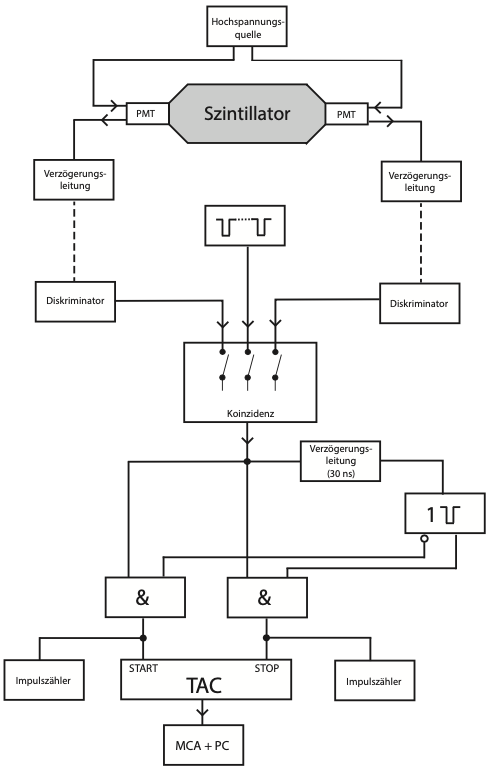
\includegraphics[width=0.7\linewidth]{figures/Aufbau.png}
    \caption{Blockschaltbild der Versuchsvorrichtung. \cite{V01}}
    \label{fig:Aufbau}
\end{figure}

\begin{figure}
    \centering
    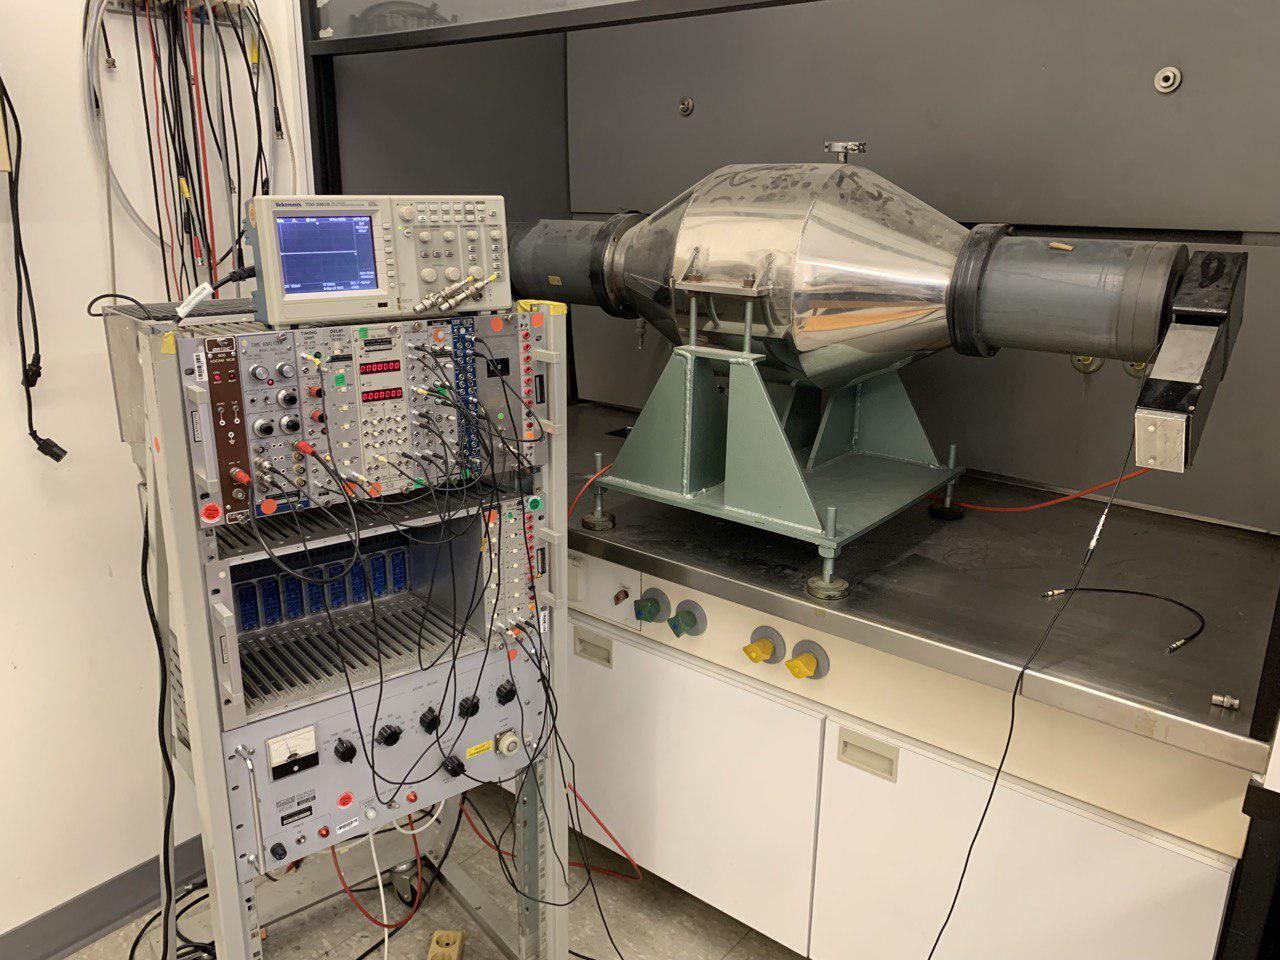
\includegraphics[width=0.7\linewidth]{figures/Aufbau_Foto.jpg}
    \caption{Foto des Versuchsaufbaus.}
    \label{fig:Aufbau_Foto}
\end{figure}

\subsection{Kalibrierung und Verkabelung}
Zunächst werden die am Szintillationstank angebrachten Photomultiplier an ein Oszilloskop angeschlossen, um sicherzustellen, dass sie funktionieren.
Anschließend werden die Photomultiplier über die Verzögerungsleitungen mit den Diskriminatoren verkabelt. Es wird noch keine Verzögerung eingestellt. Das Ergebnis wird ebenfalls am Oszilloskop sichtbar gemacht. An den Diskriminatoren wird die Pulsweite mithilfe der am Oszilloskop abgebildeten Pulse auf jeweils $\Delta t = \SI{10}{\nano\second}$ gestellt.
Als nächstes werden die Ausgänge der Diskriminatoren an einen Impulszähler angeschlossen. Die Schwelle der Diskriminatoren wird so angepasst, dass an beiden Ausgängen ca. $\num{30}$ Pulse pro Sekunde gemessen werden.
Im nächsten Schritt wird die Koinzidenz in die Schaltung integriert und der Ausgang an den Impulszähler angeschlossen. Die Verzögerungen werden systematisch nacheinander variiert. Dabei wird für jede Verzögerung die Impulsrate aufgenommen. Es ist ein deutliches Maximum, bzw. ein Plateau in der Verteilung, der Impulsrate zu sehen. Die Verzögerung wird auf diesen Wert eingestellt.
Die restliche Schaltung wird verkabelt. 
Am Monoflop wird eine Suchzeit $T_s$ eingestellt, die am auch TAC entsprechend eingestellt wird.

Der Teil vor der Koinzidenzschaltung wird abgeklemmt. Stattdessen wird ein Doppelimpulsgenerator an die Koinzidenz angeschlossen.
Die Pulsabstände werden zwischen $\SI{0.3}{\micro\second}$ und $\SI{9.9}{\micro\second}$ variiert und die entsprechende Kanalnummer des Vielkanalanalysators aufgenommen.

\subsection{Messung}
An die Koinzidenzschaltung werden erneut die zuvor abgeklemmten Photomultiplier angeschlossen. Die Aufzeichung des Vielkanalanalysators wird gleichzeitig mit dem Impulszähler gestartet und etwa $\num{20}$ bis $\SI{30}{\hour}$ laufen gelassen. %wie lange genau? Weiß man das? 